\section{Realisierung des Cloud-To-Thing Kontinuums} % (fold)
\label{sec:Realisierung des Cloud-To-Thing-Continuums}

Wie im Grundlagen Abschnitt bereits kurz erwähnt, handelt es sich beim \acrlong{cttc} um ein Bestreben, die Nutzung der Ressourcen zwischen Endgeräten und der Cloud in einem Kontinuum zu vereinen. Initiale Ansätze wurden in den letzten Jahren unter anderem von der Eclipse Foundation und dem Unternehmen ADLINK Technology entwickelt \cite{cominardiDevopsEdgeopsVision2021}. Im folgenden Abschnitt, wird das Konzept des \acrlong{cttc} im Kontext der Robotik praktisch betrachtet. Dafür wird die ebenfalls im Grundlagenabschnitt erläuterte Technologie Zenoh und ihre Stärken im Bezug auf das \acrlong{cttc} beleuchtet.

Im Hinblick auf den Robotics Bereich, ist das Protokoll Zenoh sehr Interessant. Wie im Whitepaper zum Thema Edge Computing der Eclipse Foundation \cite{cominardiDevopsEdgeopsVision2021} erwähnt, hilft dieses die Brücke zwischen den einzelnen Komponenten zu schließen. Es tut dies, indem es die Möglichkeit bietet durchgängig das gleiche Protokoll zu Nutzen. Dazu stellt es Schnittstellen in verschiedenen Sprachen bereit \cite{ZenohZeroOverhead2022}. Für Microcontroller und Embedded Devices bietet es Schnittstellen in Rust und C an. Einsteiger können dabei auf die einfacherer Python API zurückgreifen. Um Kompatibilität mit regulären HTTP-Servern zu gewährleisten, bietet Zenoh ein dazugehöriges Plugin an \cite{Eclipsezenoh}. Dieses bildet Zenoh-Pfade auf URLs ab. In Situationen, in denen ein Web Server existiert der auf Datenbanken zugreift, kann dieser Ansatz hilfreich sein. Für diese Seminararbeit von Interesse und im Folgenden näher betrachtet, ist das Zenoh Plugin für den \acrlong{dds}. Dieses ermöglicht die Integration mit Roboter die das ROS2 Betriebssystem nutzen \cite{Eclipsezenoh}. Zusammengefasst, kann man Zenoh nutzen, um zum Beispielsweise im Robotics Bereich einen direkten Zugang zu Edge und Cloud Services zu ermöglichen.\\

Ein einfaches Beispiel welches die Essenz des \acrlong{cttc} zeigt, ist die Nutzung von Sensordaten im industriellen Kontext. Zur besseren Veranschaulichung, wird das Konzept des \acrlong{cttc} anhand eines vereinfachten Beispiels dargestellt. Dieses enthält einen beweglichen Roboter, einen Steuerungsserver und eine logging Datenbank:

\begin{figure}
  \begin{center}
    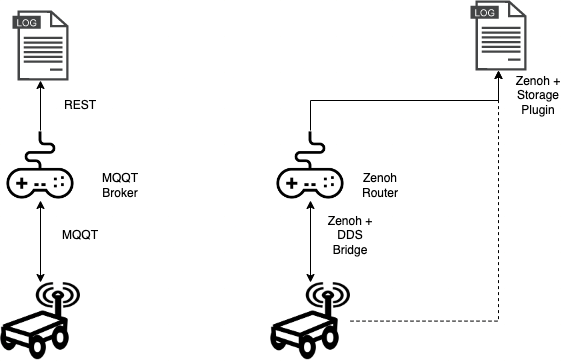
\includegraphics[width=0.5\textwidth]{./figures/cttc_demo.png}
  \end{center}
  \caption{Vereinfachtes Beispiel zur Erklärung des \acrlong{cttc}}
  \label{fig:cttc_demo}
\end{figure}

In Abbildung \ref{fig:cttc_demo} ist die zuvor beschriebene vereinfachte Architektur mit den jeweiligen Kommunikationsprotokollen dargestellt. Auf der linken Seite wird dabei MQQT für die Verbindung zwischen Roboter und Steuerungsserver genutzt. Um die Daten auf der logging Datenbank zu hinterlegen, wird eine POST-Anfrage auf eine REST-Schnittstelle getätigt.\\
Aus Sicht des vom \acrlong{cttc} angestrebten Kontinuums, ist diese Architektur nicht optimal. Durch die verschiedenen Kommunikationsprotokolle kommt es zu Unterbrechungen im Informationsfluss. Dies erhöht die Latenz sowie die Fehlerwahrscheinlichkeit durch wechselnden Technologien. Der Roboter hätte in diesem Fall auch keine Möglichkeit auf direktem Wege die logging Datenbank anzusprechen und müsste über eine Schnittstelle im Routing Server gehen. Eine Ende-Zu-Ende Kommunikation ist also nicht möglich. Dazu kommen die Eigenschaften der eingesetzten Technologien. Das MQQT-Protokoll \cite{enwiki:1127334174} wurde eingangs nicht für den Einsatz in heterogenen Umgebungen oder für die Skalierung im Zeitalter des Cloud Computings erstellt. Dazu kommt, dass die meisten MQQT-Architekturen einen Nachrichten-Broker voraussetzen und Peer-To-Peer Modelle nicht sehr häufig genutzt werden.\\

Im Vergleich zu der traditionellen Architektur, befindet sich auf der rechten Seite eine Alternative auf Basis von Zenoh die den \acrlong{cttc} Ansatz verfolgt. Zwischen dem Roboter und dem Steuerungsserver wird dabei Zenoh und eine DDS-Bridge\cite{Eclipsezenoh} genutzt. Die DDS-Bridge dient zur Übersetzung der Nachrichten vom \acrlong{dds}. Die Funktionsweise dieser wird dabei im nächsten Abschnitt \ref{sec:Integration von ROS2 mit Zenoh} näher erläutert. Für die Einbindung der logging Datenbank, kann man eine von den eingangs erwähnten Zenoh Erweiterungen nutzen die eine Schnittstelle für die externe Datenbank bietet. Es wäre hier ebenfalls möglich, über eine direkte Verbindung Nachrichten vom Roboter an die logging Datenbank zu verschicken. Eine ausführlichere Erklärung einer Peer-To-Peer Architektur wird in Abschnitt \ref{sec:Cloud und Edge Robotic Use cases} behandelt.\\
Wie man an dem Vergleich erkennen kann, erfüllt die zweite Architektur die Ansätze des \acrlong{cttc} besser als die erste. Es wird dabei eine transparente Kommunikationsstruktur ermöglicht die unabhängig von der jeweiligen Lage der Komponente erreichbar ist. Eine Skalierung in Form von weiteren Servern oder Robotern wäre hier ebenfalls einfach möglich.

% section Realisierung des Cloud-To-Thing-Continuums (end)
